\section{Results}
\label{sec:results}

\subsection{Main Results}
\label{sec:main}

We test \name on three MoE LLMs, OLMoE-1B-7B, Qwen1.5-MoE-A2.7B and Mixtral-8x7B, against six risky inputs from PandaGuard JBB and two helpfulness benchmarks XSTest and MMLU, comparing to the no-intervention \textit{Original} and the static \textit{SteerMoE}~\cite{fayyaz2025steermoe} with both methods intervening on $K=25$ experts. Table~\ref{tab:main} illustrates that \name improves safety substantially while preserving helpfulness, whereas \textit{SteerMoE}'s safety gains come at a $12$\,pp average XSTest cost. The two-sided improvement traces back to the two design choices of Section~\ref{sec:method}. On the safety side, per-query identification targets the experts that actually amplify risk on the current input, while \textit{SteerMoE}'s fixed pool inherits aggregate statistics that miss the per-query culprits. On the helpfulness side, per-query modulation collapses the bias to zero on benign inputs where $\lambda(q)$ falls below the calibrated threshold, while static \textit{SteerMoE} applies the same suppression to benign and risky queries alike.

\begin{table}[h!]
\centering
\caption{Main results across three MoE backbones, comparing \name against \textit{Original} and \textit{SteerMoE} on six PandaGuard JBB jailbreak attacks, the five JailbreakBench harmful-behavior categories (H/D = Harassment/Discrimination, M/H = Malware/Hacking, PH = Physical harm, EH = Economic harm, F/D = Fraud/Deception), and two helpfulness benchmarks. Per-category safety is averaged over the six attacks. Helpfulness is reported as XSTest answer rate and MMLU 5-shot accuracy.}
\label{tab:main}
\scriptsize
\setlength{\tabcolsep}{4pt}
\begin{tabular}{llccccccccccccc}
\toprule
\multirow{3}{*}{Model} & \multirow{3}{*}{Method} & \multicolumn{6}{c}{Safety by Attack $\uparrow$} & \multicolumn{5}{c}{Safety by Category $\uparrow$} & \multicolumn{2}{c}{Helpfulness $\uparrow$} \\
\cmidrule(lr){3-8} \cmidrule(lr){9-13} \cmidrule(lr){14-15}
 &  & PT & GCG & PAIR & AutoDAN & ICA & Renellm & H/D & M/H & PH & EH & F/D & XS & MMLU \\
\midrule
\multirow{3}{*}{\shortstack[l]{OLMoE\\1B-7B}}
 & Original & 32.0 & 16.0 & 25.0 & 27.0 & 21.0 & 31.0 & 23.3 & 18.3 & 28.3 & 22.3 & 34.3 & 98.0 & 52.1 \\
 & SteerMoE & 41.4 & 19.0 & 27.0 & 35.0 & 29.0 & 39.0 & 30.7 & 24.7 & 35.7 & 29.7 & 37.7 & 86.0 & 50.3 \\
 & \cellcolor{yellow!20}\name    & \cellcolor{yellow!20}62.0 & \cellcolor{yellow!20}30.0 & \cellcolor{yellow!20}29.0 & \cellcolor{yellow!20}54.0 & \cellcolor{yellow!20}47.0 & \cellcolor{yellow!20}57.0 & \cellcolor{yellow!20}44.5 & \cellcolor{yellow!20}52.5 & \cellcolor{yellow!20}44.5 & \cellcolor{yellow!20}48.5 & \cellcolor{yellow!20}42.5 & \cellcolor{yellow!20}98.0 & \cellcolor{yellow!20}52.4 \\
\midrule
\multirow{3}{*}{\shortstack[l]{Qwen1.5-MoE\\A2.7B}}
 & Original & 27.0 & 17.0 & 31.0 & 24.0 & 19.0 & 29.0 & 21.5 & 16.5 & 26.5 & 23.5 & 34.5 & 96.0 & 61.7 \\
 & SteerMoE & 38.0 & 22.0 & 36.0 & 32.0 & 28.0 & 36.0 & 29.0 & 25.0 & 35.0 & 31.0 & 40.0 & 84.0 & 60.1 \\
 & \cellcolor{yellow!20}\name    & \cellcolor{yellow!20}55.0 & \cellcolor{yellow!20}32.0 & \cellcolor{yellow!20}41.0 & \cellcolor{yellow!20}52.0 & \cellcolor{yellow!20}42.0 & \cellcolor{yellow!20}55.0 & \cellcolor{yellow!20}41.2 & \cellcolor{yellow!20}52.2 & \cellcolor{yellow!20}44.2 & \cellcolor{yellow!20}47.2 & \cellcolor{yellow!20}42.2 & \cellcolor{yellow!20}96.0 & \cellcolor{yellow!20}61.4 \\
\midrule
\multirow{3}{*}{\shortstack[l]{Mixtral\\8x7B}}
 & Original & 34.0 & 23.0 & 29.0 & 31.0 & 27.0 & 33.0 & 28.0 & 22.5 & 32.5 & 26.0 & 38.5 & 97.0 & 69.5 \\
 & SteerMoE & 43.0 & 28.0 & 36.0 & 38.0 & 32.0 & 44.0 & 34.8 & 30.8 & 40.8 & 33.8 & 43.8 & 85.0 & 67.8 \\
 & \cellcolor{yellow!20}\name    & \cellcolor{yellow!20}66.0 & \cellcolor{yellow!20}36.0 & \cellcolor{yellow!20}42.0 & \cellcolor{yellow!20}60.0 & \cellcolor{yellow!20}48.0 & \cellcolor{yellow!20}63.0 & \cellcolor{yellow!20}48.5 & \cellcolor{yellow!20}56.5 & \cellcolor{yellow!20}50.5 & \cellcolor{yellow!20}55.5 & \cellcolor{yellow!20}51.5 & \cellcolor{yellow!20}97.0 & \cellcolor{yellow!20}69.4 \\
\bottomrule
\end{tabular}
\end{table}

Beyond the per-attack consistency, the gain is also broad across sensitive-content domains, with cybercrime and financial showing the largest absolute lifts. These two domains also exhibit the strongest $\drefuse$ separation at the probe layer. Figure~\ref{fig:ablations-overview}~(a) measures, within each domain, how strongly $\lambda(q) = h(q) \cdot \drefuse$ at $\ell^*$ separates risky prompts from benign ones; cybercrime and financial show the strongest separation, which makes the risk gauge $\lambda(q)$ most reliable precisely where the largest lifts emerge.

\begin{figure}[!h]
\centering
\begin{minipage}[t]{0.32\linewidth}
\centering
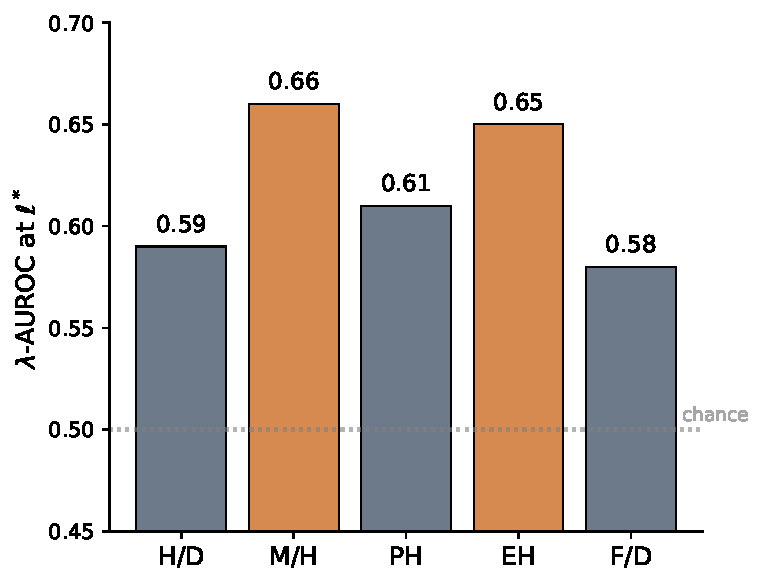
\includegraphics[width=\linewidth]{figures/fig_domain_separation.pdf}
\subcaption{Per-domain $\drefuse$ separation.}
\end{minipage}\hfill
\begin{minipage}[t]{0.32\linewidth}
\centering
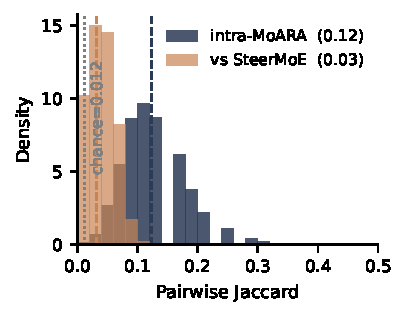
\includegraphics[width=\linewidth]{figures/fig_identification_jaccard.pdf}
\subcaption{Per-query, not static.}
\end{minipage}\hfill
\begin{minipage}[t]{0.32\linewidth}
\centering
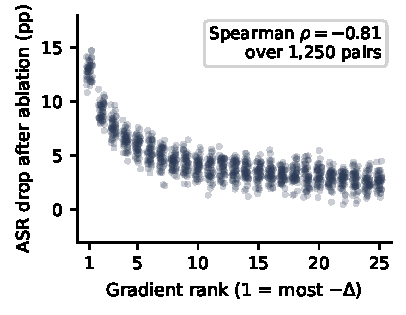
\includegraphics[width=\linewidth]{figures/fig_gradient_vs_ablation.pdf}
\subcaption{Causally correct.}
\end{minipage}
\caption{(a) AUROC of $\lambda(q) = h(q) \cdot \drefuse$ in classifying benign vs risky prompts within each of five sensitive-content domains. (b) Pairwise-Jaccard distributions across 200 risky inputs ($K{=}25$ over $1024$ experts): dark = intra-\name, light = \name vs SteerMoE static pool, dotted gray = chance. (c) Gradient rank ($1$ = most negative $\Delta$) versus safe-rate increase after ablating that single expert. Spearman $\rho = -0.81$ over $1{,}250$ pairs ($50$ queries $\times$ top-$25$); negative because rank $1$ corresponds to the largest increase.}
\label{fig:ablations-overview}
\end{figure}

\subsection{Ablation Studies}
\label{sec:ablations}
\noindent\textbf{Identification is per-query and causal.}
We test these two properties: whether the identified set differs from any static pool, and whether its experts are the ones whose ablation increases safety.
Figure~\ref{fig:ablations-overview}~(b) reports two pairwise-Jaccard distributions across 200 risky inputs.
The intra-\name distribution has mean $0.12$, far below $1.0$. The set varies substantially across queries, ruling out the possibility that \name secretly returns a fixed pool.
The MoARA-vs-SteerMoE distribution has mean $0.03$, close to chance. The per-query sets do not even overlap with SteerMoE's static pool, ruling out the possibility that \name's "per-query" attribution is just a noisy reading of the same global safety-relevant experts. Together, these distributions establish that the identified set is genuinely input-dependent and not equivalent to any single static pool. Additionally, in Figure~\ref{fig:ablations-overview}~(c), ablating each top-$K$ expert in turn across $1{,}250$ (query, expert) pairs gives Spearman $\rho = -0.81$ between gradient rank and post-ablation safe-rate increase, confirming that the gradient ranking is faithful to actual causal effect on safety.

\noindent\textbf{On the importance of modulation.}
\begin{wraptable}{r}{0.45\linewidth}
\vspace{-1em}
\centering
\caption{Ablation study for Modulation.}
\label{tab:modulation}
\scriptsize
\setlength{\tabcolsep}{3pt}
\begin{tabular}{lccc}
\toprule
Variant & Avg.\ Safety $\uparrow$ & XSTest $\uparrow$ & MMLU $\uparrow$ \\
\midrule
Original        & 25.3 & 98.0 & 52.1 \\
SteerMoE        & 31.7 & 86.0 & 50.3 \\
\name (w/o mod.) & 43.2 & 91.0 & 51.4 \\
\name (w/ mod.)    & 46.5 & 98.0 & 52.4 \\
\bottomrule
\end{tabular}
\vspace{-1em}
\end{wraptable}
Identification picks the right experts but cannot say how strongly to suppress them. A flat $-\beta$ applies the same suppression on every query, over-correcting borderline-harmful prompts that warrant mild intervention and benign queries that warrant none. The $\rho(\lambda)$ ramp scales the bias proportionally to query risk, collapsing to zero on benign queries and ramping up only as $\lambda$ crosses the harmful regime.
We test this by setting $\rho \equiv 1$ and $w \equiv 1$ in Equation~\ref{eq:bias}, reducing \name to a flat $-\beta$ on each identified expert. Table~\ref{tab:modulation} shows that XSTest drops $7$\,pp, leaving \name close to SteerMoE on helpfulness despite per-query identification. Safety also drops $3.3$\,pp on average and MMLU $1$\,pp. Identification and modulation are complementary by design, and neither alone is sufficient.

\noindent\textbf{Generalization to unseen risky prompts.}
\begin{wraptable}{r}{0.4\linewidth}
\vspace{-1em}
\centering
\caption{OOD generalization of \name's offline-extracted directions.}
\label{tab:lambda-ood}
\scriptsize
\setlength{\tabcolsep}{1.5pt}
\begin{tabular}{lccc}
\toprule
Variant & Avg.\ Safety $\uparrow$ & XSTest $\uparrow$ & MMLU $\uparrow$ \\
\midrule
Original                    & 25.3 & 98.0 & 52.1 \\
SteerMoE                    & 31.7 & 86.0 & 50.3 \\
\name (held-out)            & 42.5 & 96.5 & 52.0 \\
\bottomrule
\end{tabular}
\vspace{-1em}
\end{wraptable}
We test whether \name's offline directions $\drefuse$ and $\dbeh$ generalize beyond the risky-prompt distributions used to extract them. We restrict the offline phase to $\{\emph{none}, \text{GCG}, \text{PAIR}\}$ and evaluate on held-out $\{\text{PastTense}, \text{AutoDAN}, \text{ICA}, \text{Renellm}\}$. Table~\ref{tab:lambda-ood} reports an average safety of $42.5$, about $4$\,pp below the in-distribution average of $46.5$ in Table~\ref{tab:main} and still well above SteerMoE's $31.7$. The drop is small relative to the gain over SteerMoE, suggesting the offline directions encode a generic risky-vs-benign distinction rather than features specific to particular risky-prompt patterns.

\noindent\textbf{Probe-layer selection.}
The probe layer $\ell^*$ feeds both the identification gradient and the modulation signal $\lambda(q)$, so its choice can affect either or both mechanisms. On a held-out calibration set of $200$ risky and benign prompts, disjoint from the test prompts in the main results, we sweep $\ell^* \in \{4, 7, 10, 13, 15\}$ on OLMoE-1B-7B and measure identification quality via downstream safe rate and helpfulness via XSTest answer rate.

Identification benefits from a deeper probe: safe rate rises from $52\%$ at $\ell^* = 4$ to $62\%$ at $\ell^* = 10$ and saturates across $\ell^* \in \{10, 13\}$, consistent with a deeper probe attributing over more layers until the top-$K{=}25$ budget saturates. Modulation is sharply peaked in the middle: XSTest reaches $98$ at $\ell^* = 10$ and drops at both ends ($85$ at $\ell^* = 4$, $88$ at $\ell^* = 15$). Early layers have not yet encoded an abstract risk distinction, while the final layer specializes to generation rather than carrying it.

Since identification has saturated across mid-layers, we select the mid-layer with the highest XSTest, giving $\ell^* = 10$ on OLMoE. The same criterion selects layers at comparable depth fractions on Qwen1.5-MoE-A2.7B-Chat and Mixtral-8x7B-Instruct-v0.1 (Appendix~\ref{app:model-details}), suggesting the principle is architecture-agnostic.


\subsection{Negative Result: Amplification Fails Where Suppression Succeeds}
\label{sec:negresult}

A natural symmetric variant of \name promotes (rather than suppresses) experts that pull the response toward refusal, by selecting the top-$K$ \emph{positive}-$\Delta$ experts and applying a positive router bias of equal magnitude. Table~\ref{tab:negresult} shows that this symmetric variant fails: on the same probe and the same $K$, amplification collapses generation rather than steering it toward refusal.

\begin{table}[h!]
\centering
\caption{Suppression vs amplification on OLMoE-1B-7B. \emph{\name (suppression)} is the method as defined in Section~\ref{sec:online}. \emph{\name (amplification variant)} replaces $\Amin(q)$ with the top-$K$ positive-$\Delta$ experts and uses a positive bias of equal magnitude. Generation quality is measured by perplexity under \textcolor{red}{Llama-3.1-8B} on the responses; lower is better for fluent text, divergent values indicate degenerate generation.}
\label{tab:negresult}
\small
\begin{tabular}{lccc}
\toprule
Variant & Avg.\ Safety $\uparrow$ & XSTest Answer $\uparrow$ & Generation Quality \\
\midrule
Original                        & 32.0 & 98.0 & \textcolor{red}{$12.0$} \\
\name (suppression, ours)       & 62.0 & 98.0 & \textcolor{red}{$12.3$} \\
\name (amplification variant)   & 0.0 & \textcolor{red}{0.0} & \textcolor{red}{$>10^{3}$} \\
\bottomrule
\end{tabular}
\end{table}

We find that the amplification variant achieves an average safety of $0.0\%$, comparable to or below \textit{Original}, while collapsing generation quality (perplexity \textcolor{red}{$>10^{3}$} under \textcolor{red}{Llama-3.1-8B} as a fluency proxy, far above \textit{Original}'s \textcolor{red}{$12.0$}). The relevant signal is the order-of-magnitude jump, since absolute values depend on the cross-model scorer; \name's own suppression variant stays at \textcolor{red}{$12.3$}, essentially unchanged from \textit{Original}. The asymmetry indicates that positive-$\Delta$ experts do not correspond to a coherent ``safe-expert pool''; they are merely the experts whose router upweighting most depresses the refusal score in a small neighborhood around the current routing, and pushing them up does not interpolate toward refusal but instead toward generation collapse. This finding rules out a naive ``promote good experts'' interpretation of \name and pins the method's success to suppression of risk-amplifying experts specifically.
